%%%%%%%%%%%%%%%%%%%%%%%%%%%%%%%%%%%%%%%%%
% Short Sectioned Assignment LaTeX Template Version 1.0 (5/5/12)
% This template has been downloaded from: http://www.LaTeXTemplates.com
% Original author:  Frits Wenneker (http://www.howtotex.com)
% License: CC BY-NC-SA 3.0 (http://creativecommons.org/licenses/by-nc-sa/3.0/)
%%%%%%%%%%%%%%%%%%%%%%%%%%%%%%%%%%%%%%%%%

%----------------------------------------------------------------------------------------
%	PACKAGES AND OTHER DOCUMENT CONFIGURATIONS
%----------------------------------------------------------------------------------------

\documentclass[paper=a4, fontsize=11pt]{scrartcl} % A4 paper and 11pt font size

% ---- Entrada y salida de texto -----

\usepackage[T1]{fontenc} % Use 8-bit encoding that has 256 glyphs
\usepackage[utf8]{inputenc}
\usepackage{fourier} % Use the Adobe Utopia font for the document - comment this line to return to the LaTeX default

% ---- Idioma --------

\usepackage[spanish, es-tabla]{babel} % Selecciona el español para palabras introducidas automáticamente, p.ej. "septiembre" en la fecha y especifica que se use la palabra Tabla en vez de Cuadro

% ---- Otros paquetes ----

\usepackage{url} % ,href} %para incluir URLs e hipervínculos dentro del texto (aunque hay que instalar href)
\usepackage{amsmath,amsfonts,amsthm} % Math packages
%\usepackage{graphics,graphicx, floatrow} %para incluir imágenes y notas en las imágenes
\usepackage{graphics,graphicx, float} %para incluir imágenes y colocarlas

% Para hacer tablas comlejas
%\usepackage{multirow}
%\usepackage{threeparttable}

%\usepackage{sectsty} % Allows customizing section commands
%\allsectionsfont{\centering \normalfont\scshape} % Make all sections centered, the default font and small caps

\usepackage{fancyhdr} % Custom headers and footers
\pagestyle{fancyplain} % Makes all pages in the document conform to the custom headers and footers
\fancyhead[L]{Práctica 2}  % Header name
\fancyhead[C]{} % Empty center header
\fancyhead[R]{Fundamentos de la Ingeniería del Software} % Header title
\fancyfoot[L]{} % Empty left footer
\fancyfoot[C]{} % Empty center footer
\fancyfoot[R]{\thepage} % Page numbering for right footer
\renewcommand{\headrulewidth}{0pt} % Remove header underlines
\renewcommand{\footrulewidth}{0pt} % Remove footer underlines
\setlength{\headheight}{10pt} % Customize the height of the header

\numberwithin{equation}{section} % Number equations within sections (i.e. 1.1, 1.2, 2.1, 2.2 instead of 1, 2, 3, 4)
\numberwithin{figure}{section} % Number figures within sections (i.e. 1.1, 1.2, 2.1, 2.2 instead of 1, 2, 3, 4)
\numberwithin{table}{section} % Number tables within sections (i.e. 1.1, 1.2, 2.1, 2.2 instead of 1, 2, 3, 4)

\setlength\parindent{0pt} % Removes all indentation from paragraphs - comment this line for an assignment with lots of text

\newcommand{\horrule}[1]{\rule{\linewidth}{#1}} % Create horizontal rule command with 1 argument of height



%----------------------------------------------------------------------------------------
%	TÍTULO Y DATOS DEL ALUMNO
%----------------------------------------------------------------------------------------

\title{	
\normalfont \normalsize 
\textsc{\textbf{Fundamentos de Ingeniería del Software (2016-2017)} \\ Grado en Ingeniería Informática \\ Universidad de Granada} \\ [25pt] % Your university, school and/or department name(s)
\horrule{2pt} \\[0.4cm] % Thin top horizontal rule
\huge Práctica 2 \\ % The assignment title
\horrule{2pt} \\[0.5cm] % Thick bottom horizontal rule
}

\author{Miguel Ángel Torres López \and Francisco José Ruiz Jiménez \and Francisco Gallego Salido \and Francisco Lopez Rodríguez} % Nombre y apellidos


\date{\normalsize\today} % Incluye la fecha actual

%----------------------------------------------------------------------------------------
% DOCUMENTO
%----------------------------------------------------------------------------------------

\begin{document}

\maketitle % Muestra el Título

\newpage %inserta un salto de página

\tableofcontents % para generar el índice de contenidos

\listoffigures

\newpage

%----------------------------------------------------------------------------------------
%	Cuestión 1
%----------------------------------------------------------------------------------------

\section{Objetivos}

Esta sección tiene como objetivo presentar y definir los casos de uso necesarios para comprender mejor el sistema planteado en la práctica 1. Al glosario de términos, 
la descripción de actores y la especificación de requisitos ahora añadimos los casos de uso y la relación de estos con los actores.

\vspace{8mm}

\section{Jerarquía de casos de uso}
\subsection{Gestión de Usuarios}
\textbf{Descripción:}\\
Escenarios asociados con acciones sobre los socios.\\
\textbf{Casos de uso:}\\
	\begin{itemize}
		\item Registro de usuario.
		\item Baja de usuario.
		\item Modificar datos de usuario.
		\item Consultar perfil de usuario.
		\item Consultar reservas actuales.
		\item Consultar historial de reservas.
		\item Añadir viviendas o vehículos al perfil.
		\item Gestionar viviendas y vehículos.
	\end{itemize}
\subsection{Gestión de Solicitudes y Reservas}
\textbf{Descripción:}\\
Escenarios asociados con la gestión de solicitudes y reservas.\\
\textbf{Casos de uso:}\\
	\begin{itemize}
		\item Solicitar/Reservar vehículo o vivenda.
		\item Cancelar solicitud.
		\item Gestionar críticas y puntuaciones de solicitantes.
		\item Adjuntar mensajes a una solicitud.
	\end{itemize}
\subsection{Gestión de Ofertas}
\textbf{Descripción:}\\
Escenarios asociados con la gestión de ofertas de usuarios.\\
\textbf{Casos de uso:}\\
	\begin{itemize}
		\item Búsqueda de ofertas.
		\item Gestión de ofertas realizadas.
		\item	Consultar disponibilidad de ofertas.
		\item Gestionar críticas y puntuaciones de solicitantes.
		\item Publicación de ofertas de vehículos y viviendas.
		\item Sesgar ofertas por preferencias.
		\item Cancelar ofertas antes de la fecha de uso.											
	\end{itemize}

\section{Diagrama de paquetes}
	\begin{figure}[H] 
		\centering
		\includegraphics[scale=0.6]{Diagrama_de_paquetes.png}  
		\caption{Diagrama de paquetes} \label{fig:figura1}
	\end{figure}
\newpage
\section{Diagramas de casos de uso}
	\subsection{Gestión de usuarios}
		\begin{figure}[h!]
			\centering
			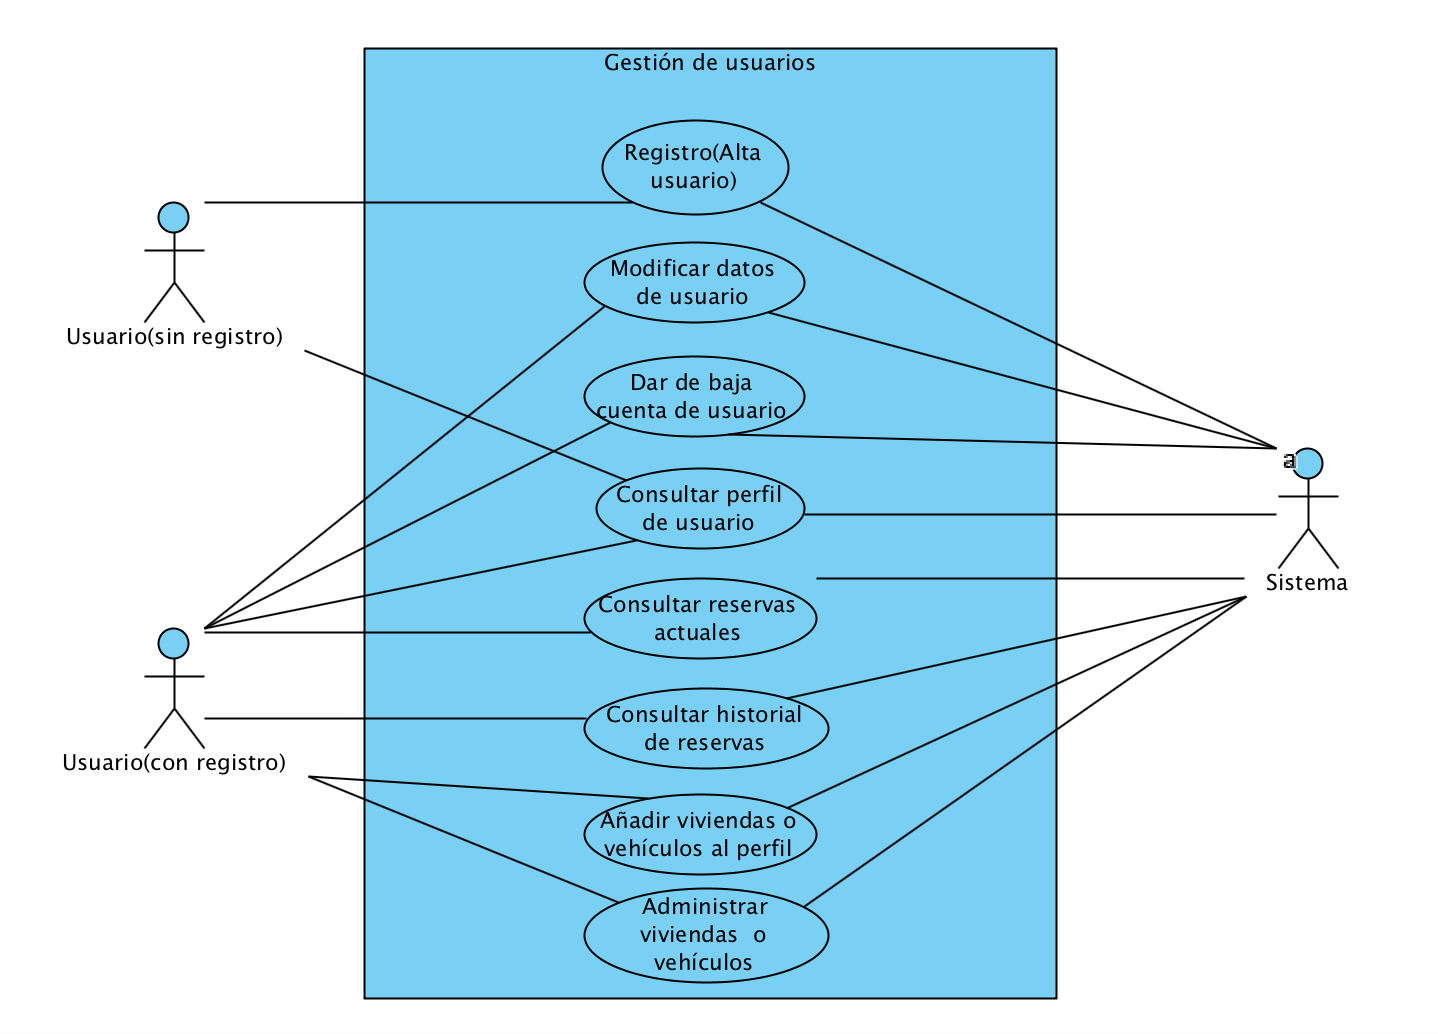
\includegraphics[width=1.15\linewidth]{Gestion_usuarios}
			\caption{diagrama gestión de usuarios}
			\label{fig:gestionusuarios}
		\end{figure}
\newpage
	\subsection{Gestión de solicitudes y reservas}
		\begin{figure}[h!]
			\centering
			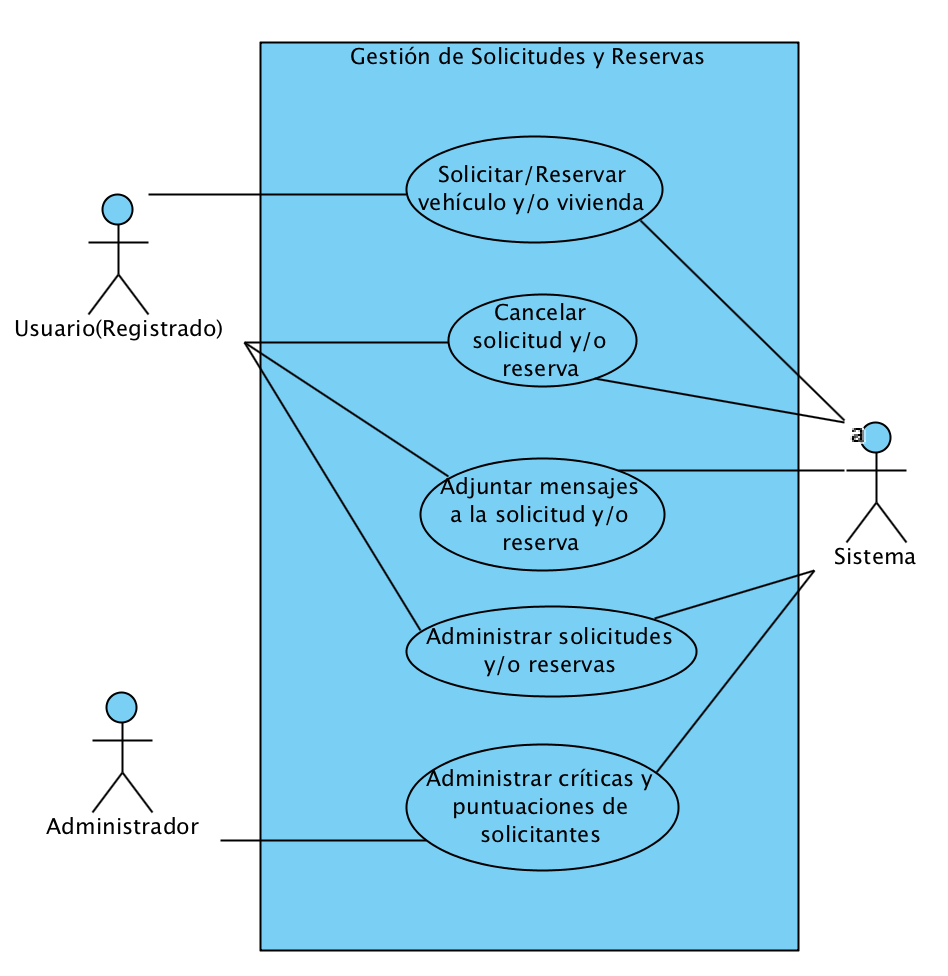
\includegraphics[width=1\linewidth]{Gestion_solicitudes_reservas}
			\caption{diagrama gestión de solicitudes y reservas}
			\label{fig:gestionsolicitudesreservas}
		\end{figure}
\newpage
	\subsection{Gestión de ofertas}
		\begin{figure}[h!]
			\centering
			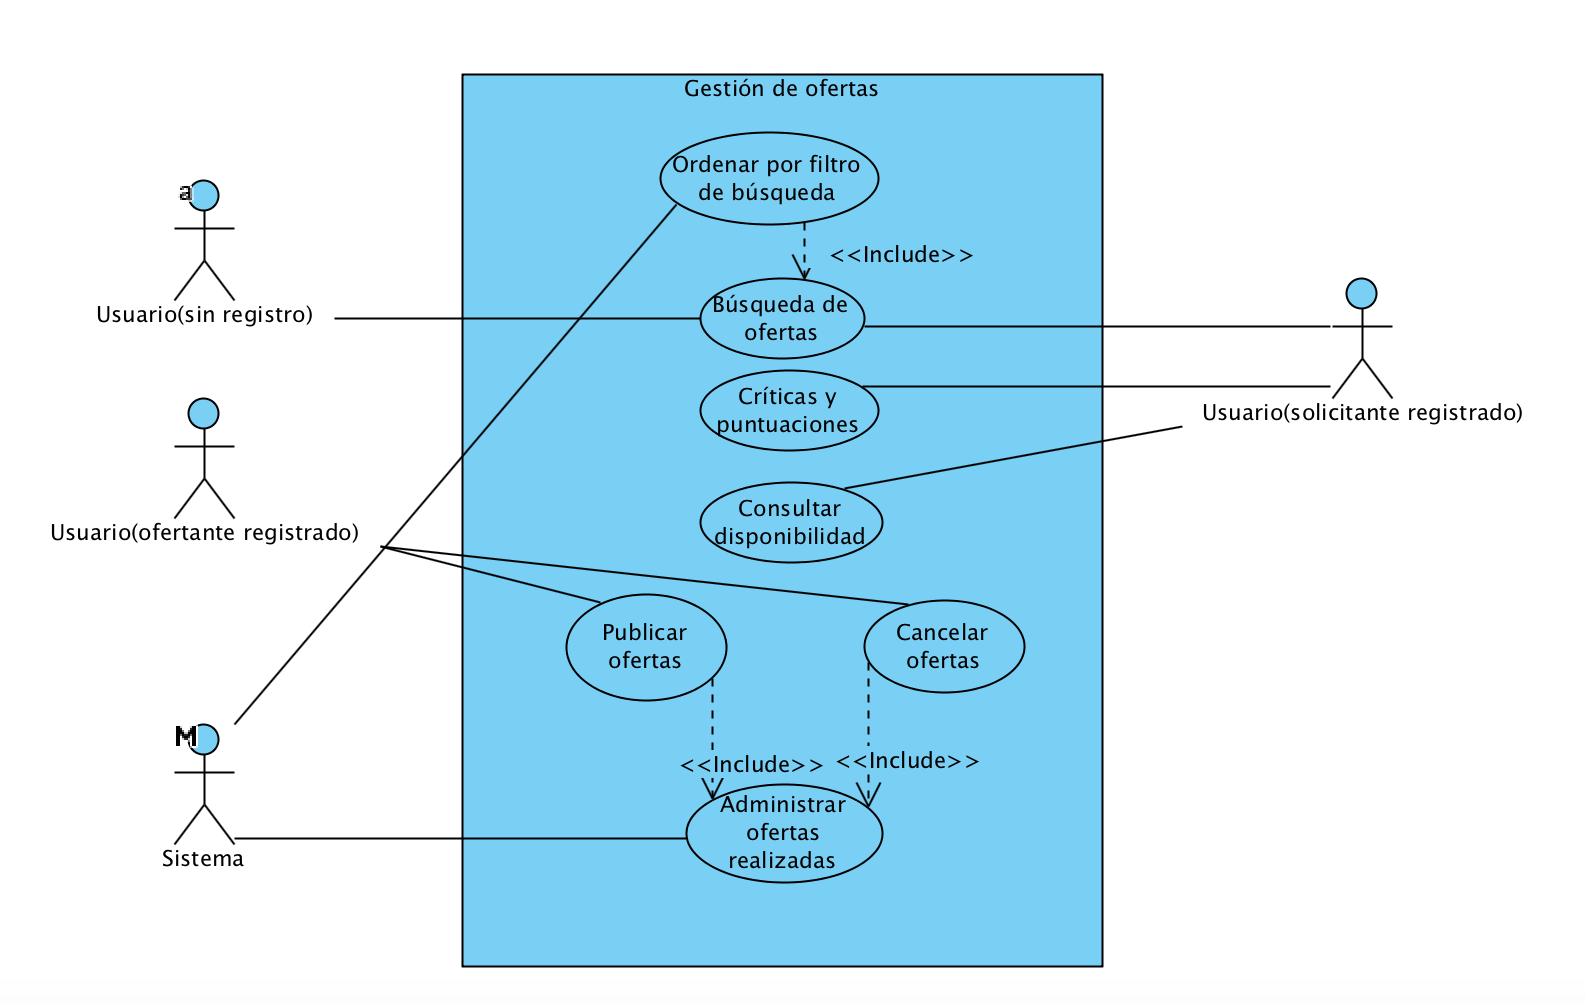
\includegraphics[width=1.2\linewidth]{Gestion_de_ofertas}
			\caption{diagrama gestión de ofertas}
			\label{fig:gestionofertas}
		\end{figure}
		
\newpage

\section{Descripción básica de casos de uso}
	\subsection{Actores}
	\vspace{-5mm}
	\begin{figure}[h!]
		\centering
		\includegraphics[width=0.78\linewidth]{img/actores/Usuario_con_registro}
		\label{fig:administrador}
	\end{figure}
	\vspace{-5mm}
	\begin{figure}[h!]
		\centering
		\includegraphics[width=0.82\linewidth]{img/actores/Usuario_sin_registro}
		\label{fig:administrador}
	\end{figure}
	\begin{figure}[h!]
		\centering
		\includegraphics[width=0.95\linewidth]{img/actores/Sistema}
		\label{fig:administrador}
	\end{figure}
	\begin{figure}[h!]
		\centering
		\includegraphics[width=0.91\linewidth]{img/actores/Usuario_ofertante}
		\label{fig:administrador}
	\end{figure}
	\begin{figure}[h!]
		\centering
		\includegraphics[width=0.95\linewidth]{img/actores/Usuario_solicitante}
		\label{fig:administrador}
	\end{figure}
	\begin{figure}[h!]
		\centering
		\includegraphics[width=0.95\linewidth]{img/actores/Administrador}
		\label{fig:administrador}
	\end{figure}
	
\clearpage

\subsection{Casos de uso}

	\begin{figure}[h!]
		\centering
		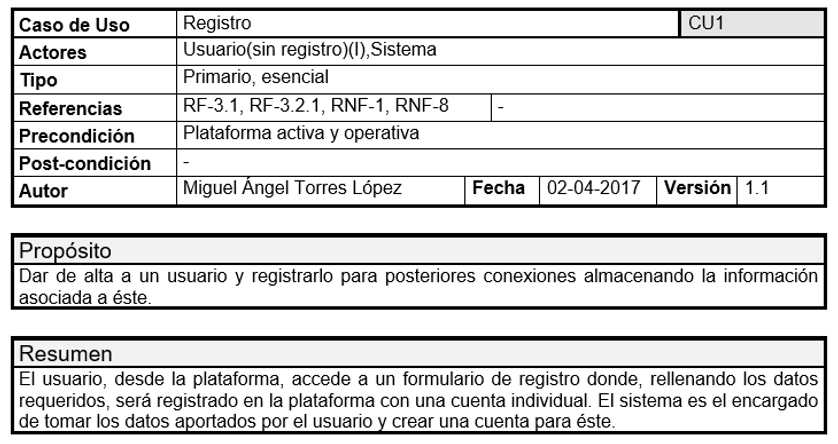
\includegraphics[width=0.95\linewidth]{img/casos/usuarios/Gestion_usuarios_registro}
		\label{fig:gestionusuariosregistro}
	\end{figure}
	
	\begin{figure}[h!]
		\centering
		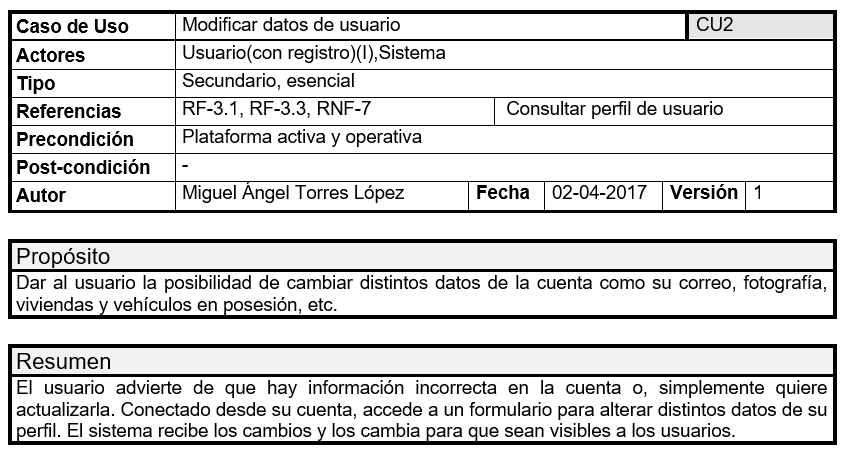
\includegraphics[width=0.94\linewidth]{img/casos/usuarios/Gestion_usuarios_modificar_datos}
		\label{fig:gestionusuariosmodificardatos}
	\end{figure}ç
\clearpage
	\begin{figure}[h!]
		\centering
		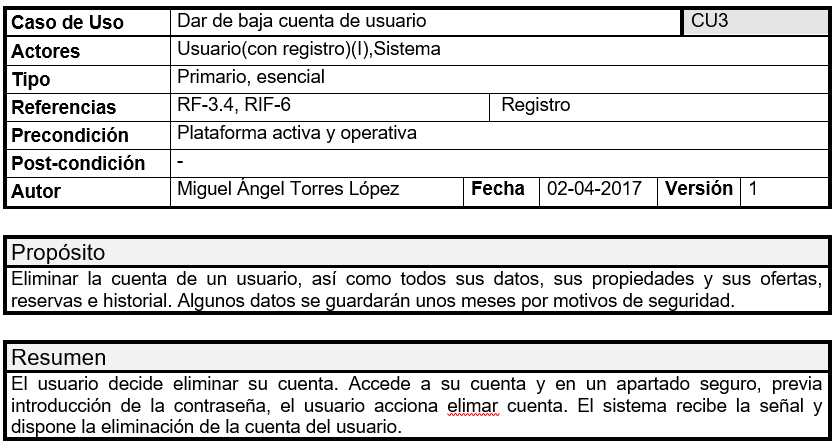
\includegraphics[width=0.95\linewidth]{img/casos/usuarios/Gestion_usuarios_dar_de_baja}
		\label{fig:gestionusuariosdardebaja}
	\end{figure}
	
	\begin{figure}[h!]
		\centering
		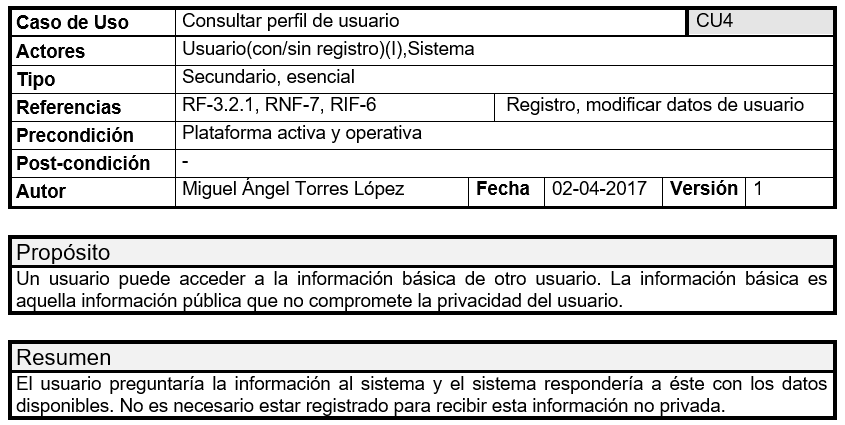
\includegraphics[width=0.95\linewidth]{img/casos/usuarios/Gestion_usuarios_consultar_perfil}
		\label{fig:gestionusuariosconsultarperfil}
	\end{figure}
\clearpage
	\begin{figure}[h!]
		\centering
		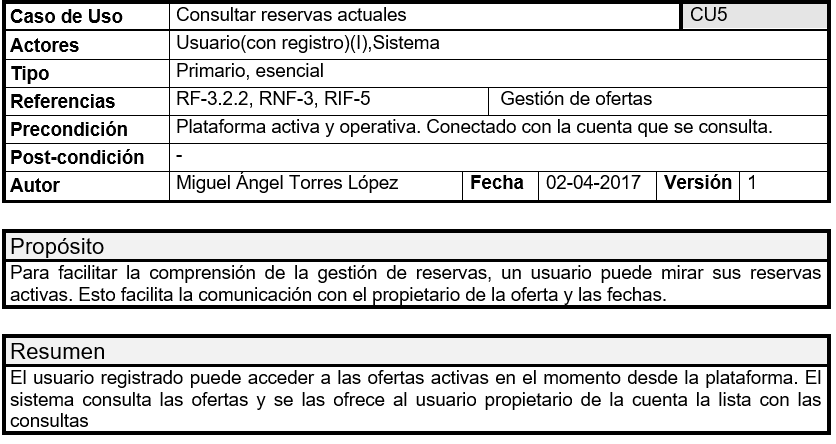
\includegraphics[width=0.9\linewidth]{img/casos/usuarios/Gestion_usuarios_consultar_reservas}
		\label{fig:gestionusuariosconsultarreservas}
	\end{figure}
			
	\begin{figure}[h!]
		\centering
		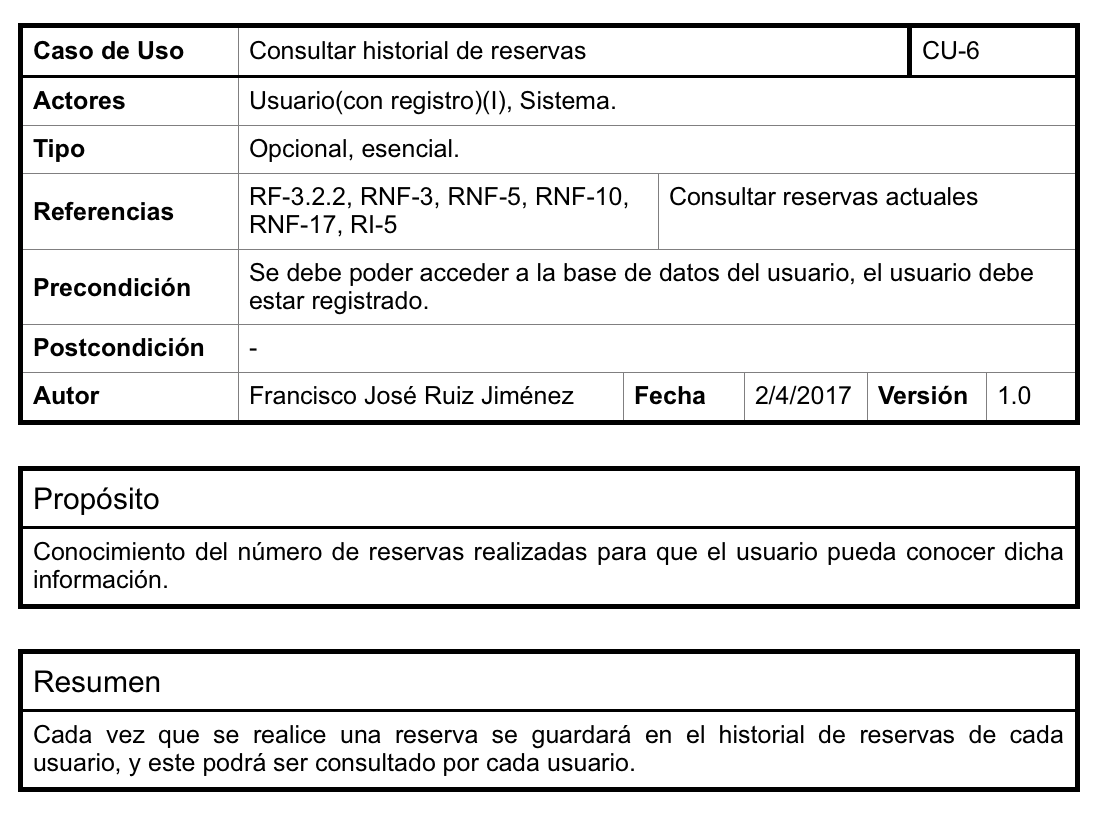
\includegraphics[width=0.9\linewidth]{img/casos/usuarios/Consulta_historial_reservasCU-6}
		\label{fig:consultahistorialreservascu-6}
	\end{figure}
\clearpage
	\begin{figure}[h!]
		\centering
		\includegraphics[width=0.9\linewidth]{img/casos/usuarios/Aniadir_vivienda_o_vehiculo_al_perfilCU-7}
		\label{fig:anadirviviendaovehiculoalperfilcu-7}
	\end{figure}
	
	\begin{figure}[h!]
		\centering
		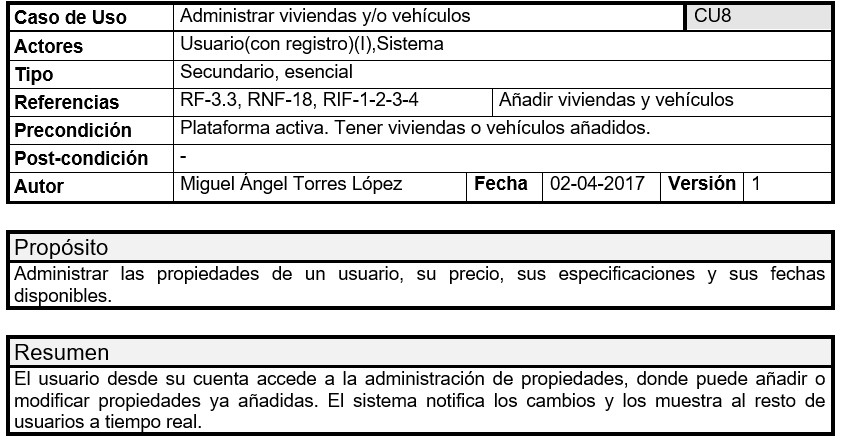
\includegraphics[width=0.9\linewidth]{img/casos/usuarios/Gestion_usuarios_administrar_propiedades}
		\label{fig:gestionusuariosadministrarpropiedades}
	\end{figure}
\clearpage
	\begin{figure}[h!]
		\centering
		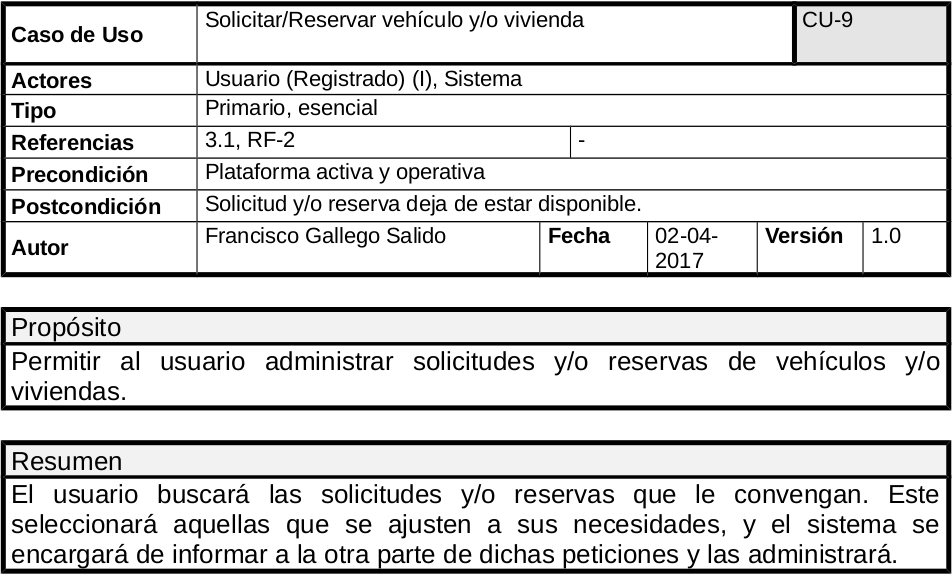
\includegraphics[width=0.9\linewidth]{img/casos/solicitudes_reservas/Caso_solicitud_reserva}
		\label{fig:casosolicitudreserva}
	\end{figure}
	
	\begin{figure}[h!]
		\centering
		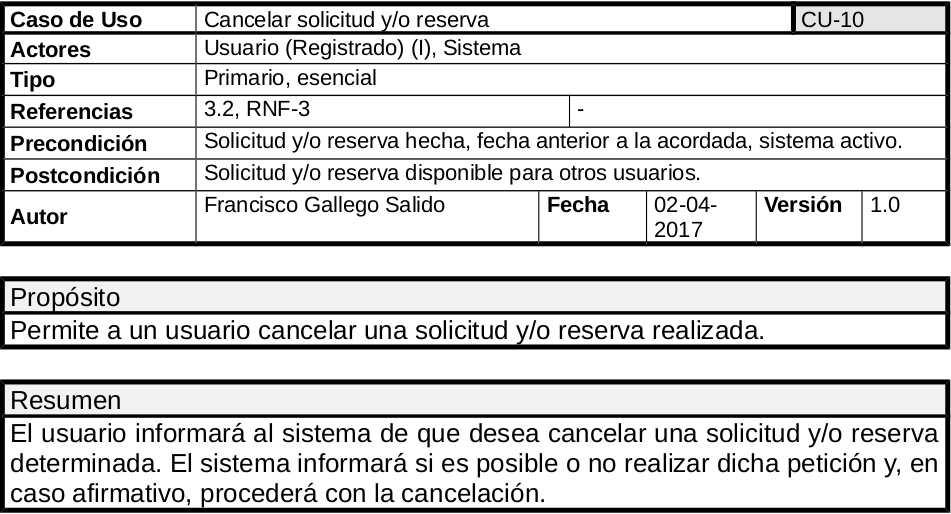
\includegraphics[width=0.9\linewidth]{img/casos/solicitudes_reservas/Caso_cancelacion_solicitudes}
		\label{fig:casocancelacionsolicitudes}
	\end{figure}
\clearpage
	\begin{figure}[h!]
		\centering
		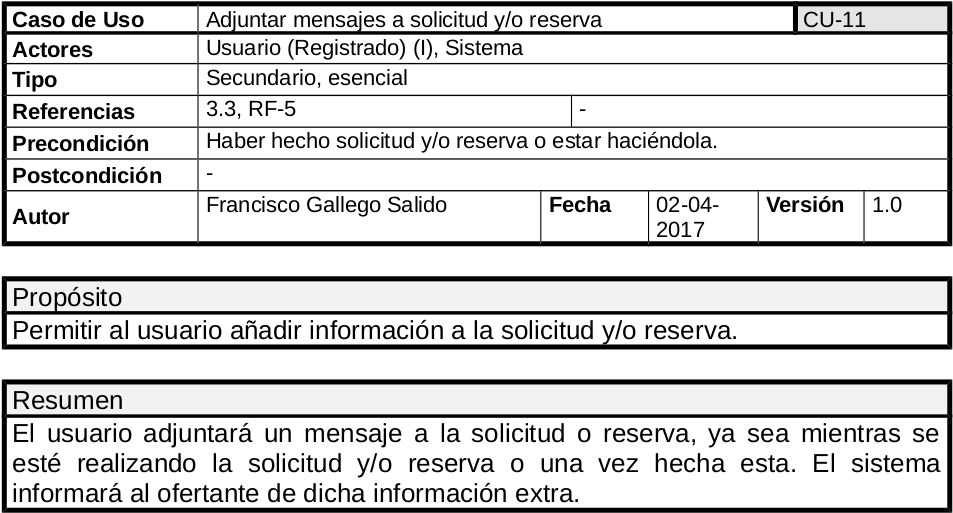
\includegraphics[width=0.9\linewidth]{img/casos/solicitudes_reservas/Caso_adjuntar_mensaje_a_solicitud}
		\label{fig:casoadjuntarmensajeasolicitud}
	\end{figure}

	\begin{figure}[h!]
		\centering
		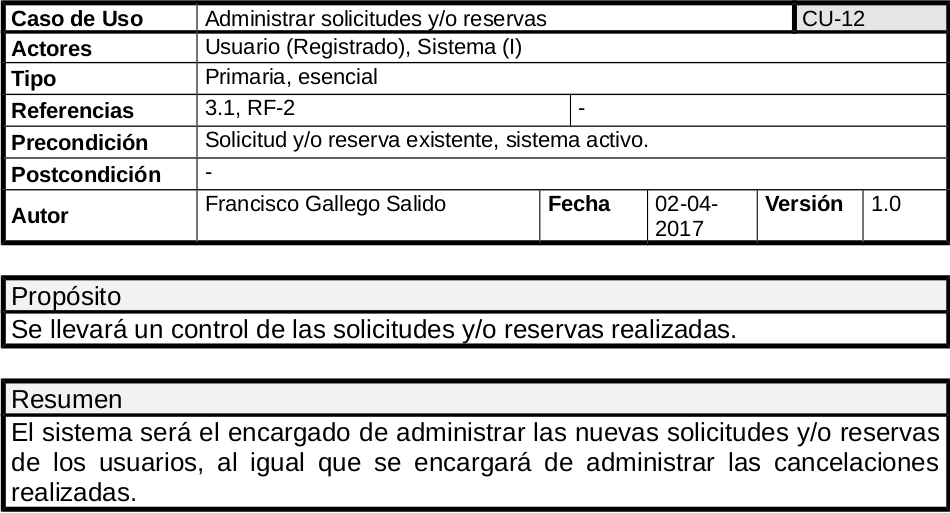
\includegraphics[width=0.9\linewidth]{img/casos/solicitudes_reservas/Caso_administrar_solicitudes}
		\label{fig:casoadministrarsolicitudes}
	\end{figure}
\clearpage
	\begin{figure}[h!]
		\centering
		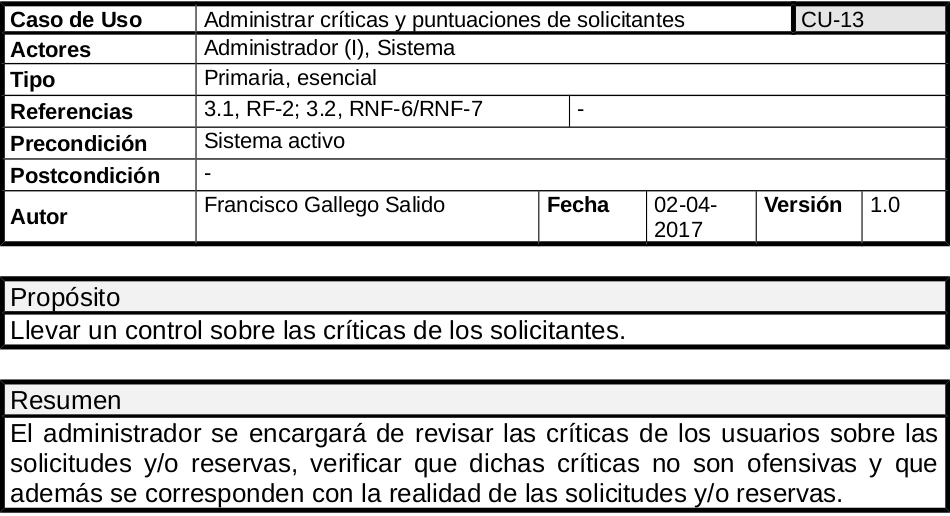
\includegraphics[width=0.9\linewidth]{img/casos/solicitudes_reservas/Caso_administrar_criticas}
		\label{fig:casoadministrarcriticas}
	\end{figure}

	\begin{figure}[h!]
		\centering
		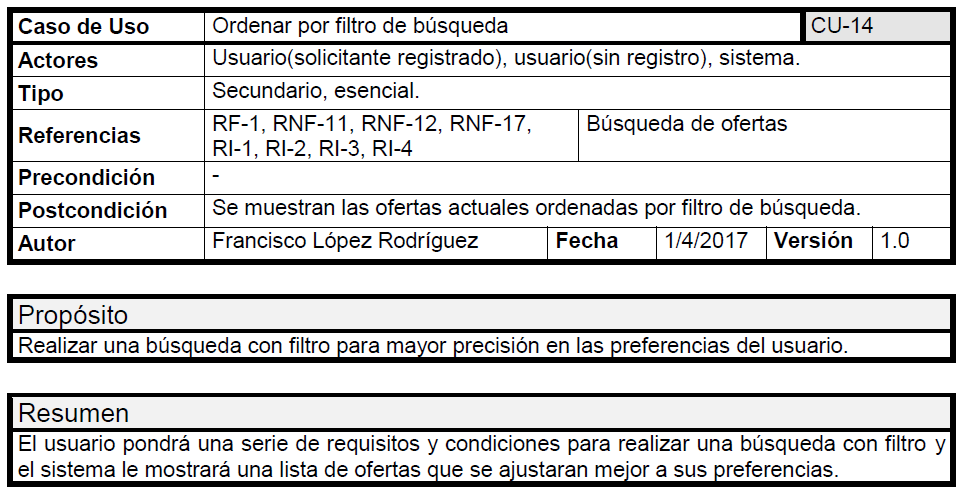
\includegraphics[width=0.9\linewidth]{img/casos/ofertas/filtro_busqueda}
		\label{fig:filtrobusqueda}
	\end{figure}
\clearpage
	\begin{figure}[h!]
		\centering
		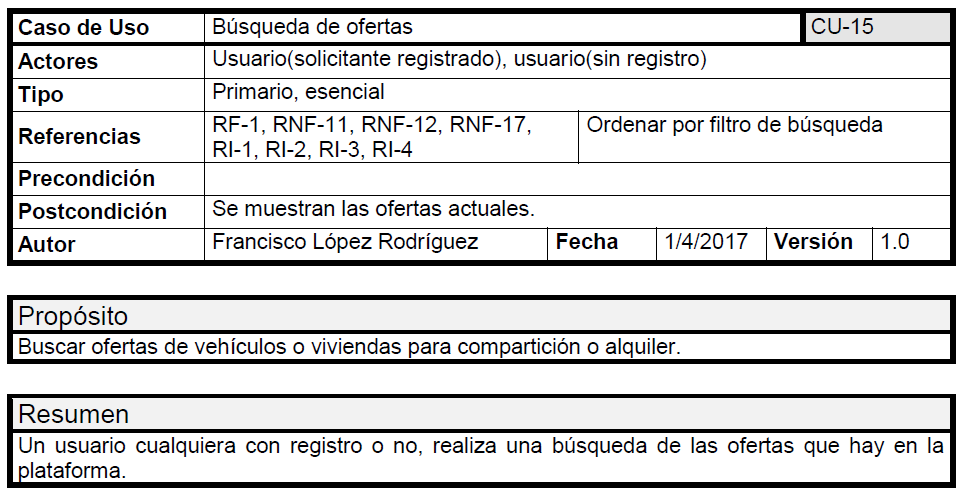
\includegraphics[width=0.9\linewidth]{img/casos/ofertas/busqueda_ofertas}
		\label{fig:busquedaofertas}
	\end{figure}
	
	\begin{figure}[h!]
		\centering
		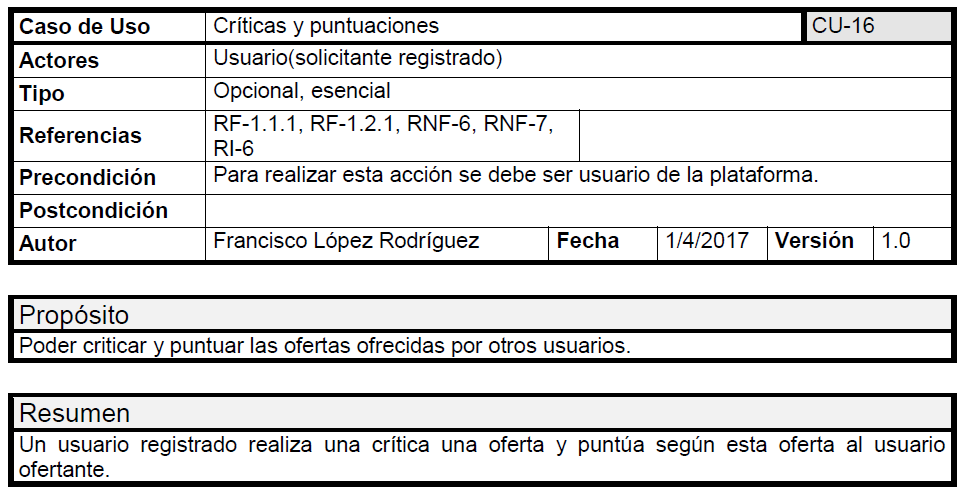
\includegraphics[width=0.9\linewidth]{img/casos/ofertas/criticas_y_puntuaciones}
		\label{fig:criticasypuntuaciones}
	\end{figure}
\clearpage
	\begin{figure}[h!]
		\centering
		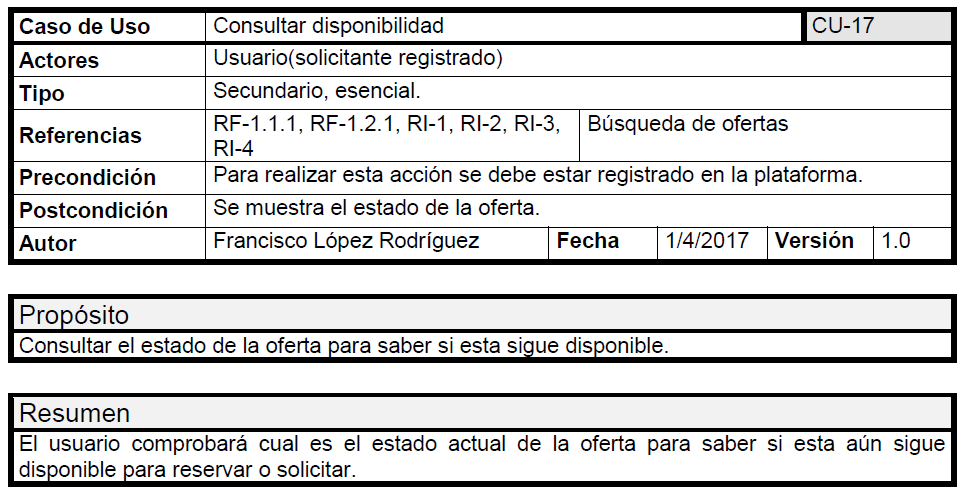
\includegraphics[width=0.9\linewidth]{img/casos/ofertas/disponibilidad}
		\label{fig:criticasypuntuaciones}
	\end{figure}
	
	\begin{figure}[h!]
		\centering
		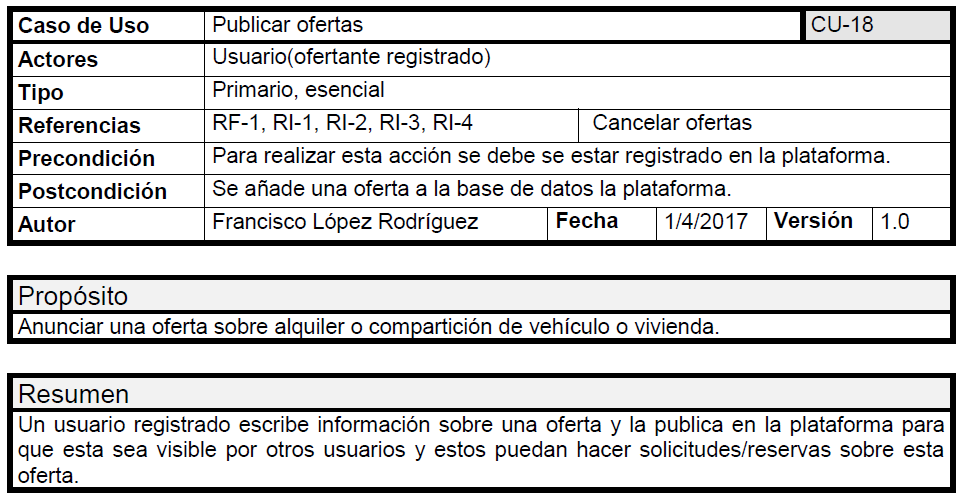
\includegraphics[width=0.9\linewidth]{img/casos/ofertas/publicar_ofertas}
		\label{fig:criticasypuntuaciones}
	\end{figure}
\clearpage
	\begin{figure}[h!]
		\centering
		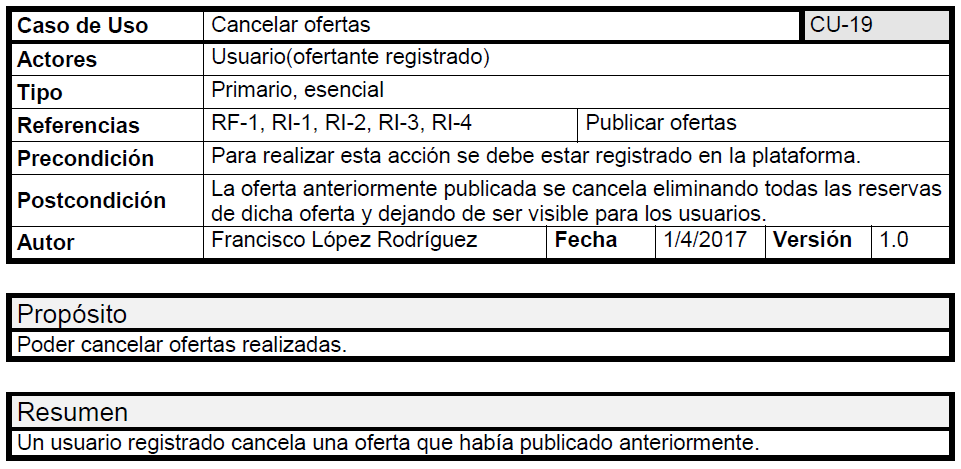
\includegraphics[width=0.9\linewidth]{img/casos/ofertas/cancelar_ofertas}
		\label{fig:criticasypuntuaciones}
	\end{figure}
	\begin{figure}[h!]
		\centering
		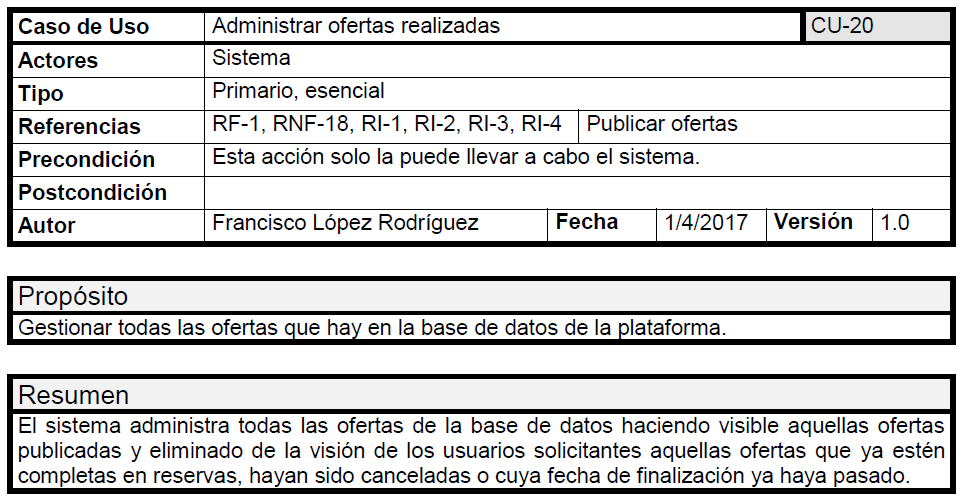
\includegraphics[width=0.9\linewidth]{img/casos/ofertas/administrar_ofertas}
		\label{fig:criticasypuntuaciones}
	\end{figure}
\end{document}


